\documentclass[10pt,twocolumn]{article}
\usepackage[a4paper,margin=1in]{geometry, graphicx, hyperref}
\usepackage{float}
\raggedbottom
\usepackage[
style=ieee,
sorting=none,
]{biblatex}
\usepackage{amsmath}
\usepackage{footnotebackref}
\usepackage{enumitem}
\usepackage[skip=1pt]{caption}
\usepackage{xcolor}
\hypersetup{
    colorlinks,
    linkcolor={red!80!black},
    citecolor={blue!50!black},
    urlcolor={blue!80!black}
}
\usepackage{mathtools}
\usepackage{amsfonts}
\addbibresource{sample.bib}

\title{\textbf{Topological Analysis of Goal Scoring Patterns using Passing Networks}}
\author{Mert Bildirici, Sam Borremans, Lauren Liu}
\date{\href{https://github.com/Sam-B-Y/TDA-Soccer-Passing-Networks}{github.com/Sam-B-Y/TDA-Soccer-Passing-Networks}}

\begin{document}

\maketitle

\section*{Introduction}
At the heart of a soccer team's strategy and performance is its passing network — a web of interactions that reflects how players connect and collaborate on the field. These networks hold valuable information about a team's style of play, major contributors, and overall effectiveness. 

To uncover deeper structural patterns within these networks, Topological Data Analysis (TDA) can be used to study the ``shape" of data by identifying its inherent patterns and structures. TDA has been successfully applied in sports like basketball \cite{roehm-2021} and hockey \cite{goldfarb-2014}, where passing is crucial, offering valuable insights into team dynamics and performance. 

With the growing application of data science in soccer \cite{lolli-2024}, and particularly in analyzing passing networks \cite{buldu-2018}, we wanted to explore how the topology of soccer teams' networks — especially their homology — correlates with their scoring. By examining these relationships, this study seeks to provide insights into passing strategies that can enhance goal-scoring outcomes in soccer.

This paper will look at the 2015/2016 season across Europe's top five leagues: the Premier League, the Bundesliga, Serie A, La Liga, and Ligue 1. It first introduces the construction and interpretation of passing networks, followed by an overview of the TDA applications employed. Finally, it analyzes the relationship between the homology of passing networks and the number of goals scored by a team, while also providing insights into the differences across these five leagues.

\section*{Passing Networks}

The construction of these networks starts with raw match data, which we pulled from StatsBomb \cite{statsbomb-no-date}. They collect passing data by using computer vision to track the ball's movement during a match, before manually verifying the data with human analysts \cite{hudl-statsbomb-data-champions-2024}. Their data includes the location of the pass origin and destination, as well as the involved players, the type of pass, and the number of goals. Their data is free for certain games, including all games in the 2015/2016 season, which is why we chose to focus on these for this paper.

Players are represented as nodes, and the edges between nodes represent the passes between two players. Their weight will depend on how many passes those two players passed to each other successfully during the game. 

\begin{figure}[H]
    \centering
    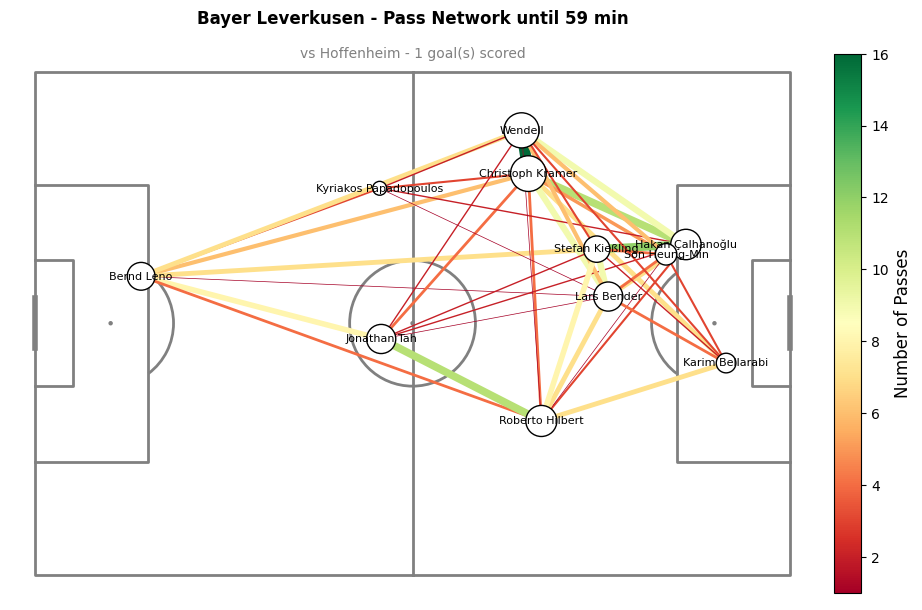
\includegraphics[width= 1 \linewidth]{images/leverkusen.png}
    \caption{Example Passing Network Graph for Bayer Leverkusen}
    \label{fig:leverkusen}
\end{figure}


\section*{Persistence}

A \textit{filtration} examines the evolution of a network's topology as a threshold parameter gradually increases, revealing features like connected components and loops at different scales. To apply filtration to our dataset an inverted weighting scheme is adopted: unlike traditional passing networks where stronger connections are associated with higher weights, the more frequent the passes between two players, the lower the weight of the edge connecting their nodes.  By inverting the weights, frequent passes (which signify stronger player relationships) appear first and persist longer, allowing us to capture the team's core structure in the early stages of filtration. In the context of our passing network, the filtration thus represents the inverse of an amount of passing, revealing weaker connections between players as the threshold parameter increases.

A \textit{simplicial complex} is a set of simplices — points, line segments, triangles, and their higher-dimensional counterparts — that satisfies the property that every face of a simplex is also in the complex, and the intersection of any two simplices is either empty or a lower-dimensional simplex. Tracking the homology groups of these complexes as the threshold changes reveals when particular topological features are ``birthed" and when they ``die". Thus, to quantify the structure of passing networks, we construct a \textit{persistence diagram}, which encodes the birth and death of topological features as a filtration parameter increases. By gradually ``thickening" the network we obtain a sequence of nested simplicial complexes. This sequence is the filtration we defined above.  \cite{aktas-2019}.


Formally, let $ G = (V, E, w) $ be the weighted graph representing the passing network, where $ V $ is the set of players, $ E \subseteq V \times V $ is the set of edges, and $ w: E \to \mathbb{R} $ assigns each edge \(e \in E\) a weight based on the frequency of passes between the players. The edge weight $ w(e) $ between players $ i $ and $ j $ is calculated using the formula:

\[
w(e_{ij}) = 
\begin{cases} 
1 - \frac{\text{count}_{ij} - \min(\text{count})}{\max(\text{count}) - \min(\text{count})} & \text{if } \text{count}_{ij} \neq 0 \\
\infty & \text{if } \text{count}_{ij} = 0
\end{cases}
\]

where $ \text{count}_{ij} $ is the number of passes between players $ i $ and $ j $, and $ \min(\text{count}) $ and $ \max(\text{count}) $ are the minimum and maximum pass counts across all pairs of players in the team for that match, respectively. By normalizing the weights, we can compare filtration across different games of different lengths. Two players who have never passed the ball to each other should not have an edge between them. We thus assigned such nonexistent edges a weight of infinity to exclude them from the filtration process.

Next, let us define a filtration parameter $\epsilon \in \mathbb{R}$. For each $\epsilon$, consider the subgraph  
\[
G_\epsilon = (V, E_\epsilon), \quad \text{where } E_\epsilon = \{ e \in E \mid w(e) \leq \epsilon \}.
\]

To form a simplicial complex from a graph, we utilize the \textit{Vietoris-Rips complex} construction. The Vietoris-Rips complex includes a simplex for any finite set of vertices where the pairwise distances (edge weights) are all below the threshold $\epsilon$. For each $\epsilon$, we construct the Vietoris-Rips complex $ VR_\epsilon $ defined as:
\[
VR_\epsilon = \{ \sigma \subseteq V \mid \forall i, j \in \sigma, \ e_{ij} \in E \Rightarrow w(e_{ij}) \leq \epsilon \}.
\]
If an edge $ e_{ij} $ is not present in $ E $ (i.e., $ w(e_{ij}) = \infty $), then any simplex containing both $ i $ and $ j $ will not be included in $ VR_\epsilon $ for any finite $\epsilon$.

As $\epsilon$ increases, we obtain a nested sequence of simplicial complexes:
\[
VR_{\epsilon_1} \subseteq VR_{\epsilon_2} \subseteq \cdots \subseteq VR_{\epsilon_m}.
\]

From each complex $VR_{\epsilon_i}$, we compute the homology groups $H_k(VR_{\epsilon_i}; \mathbb{F})$ over a field $\mathbb{F}$ (commonly $\mathbb{F}=\mathbb{Z}_2$). The $k$-th homology group is given by:
\[
H_k(VR_{\epsilon_i}; \mathbb{F}) = \frac{\ker(\partial_k)}{\mathrm{im}(\partial_{k+1})},
\]
where $\partial_k : C_k(VR_{\epsilon_i}) \to C_{k-1}(VR_{\epsilon_i})$ is the boundary map on the $k$-th chain group. These homology groups detect topological features of dimension $k$: connected components ($k=0$), loops ($k=1$), and higher-dimensional voids ($k \geq 2$).

Persistent homology tracks these homology groups across the filtration. A topological feature (such as a loop) that is born at scale $\epsilon_b$ and dies at scale $\epsilon_d$ is represented as a point $(\epsilon_b, \epsilon_d)$ in the persistence diagram:
\[
Dg_k = \{(\epsilon_b, \epsilon_d) \mid \text{feature in } H_k(VR_{\epsilon}) \text{ for } \epsilon \in [\epsilon_b,\epsilon_d)\}.
\]

This can be visualized by the following graph, representing the persistence diagram of the game in Figure \ref{fig:leverkusen}:

\begin{figure}[H]
    \centering
    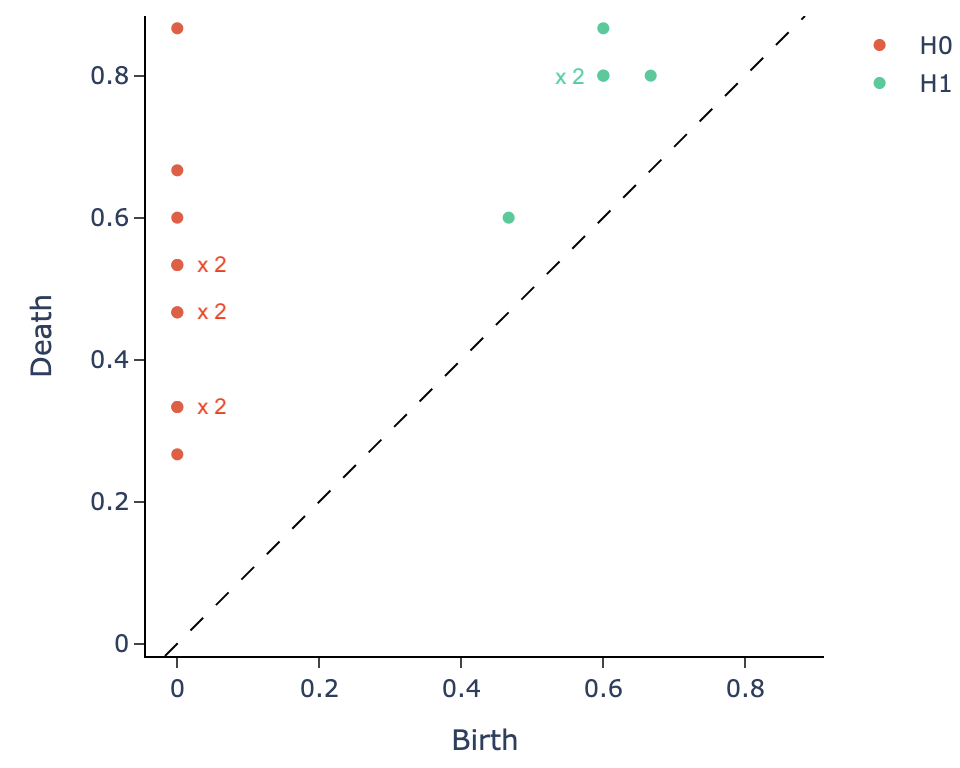
\includegraphics[width=0.8\linewidth]{images/birthdeath.png}
    \caption{Example Persistence Diagram for a Team in a Single Game}
    \label{fig:persistence_diagram}
\end{figure}

All players, represented by the $H_0$ data points, are birthed at 0 as no passes are required for them to appear in our network. Features in $H_1$ representing passing loops need at least three edges to form, and are therefore birthed later.

We can note that some of these points have high multiplicity, as nodes and edges ``die" at the same time with the simultaneous apparition of edges. Accounting for the multiplicity, this diagram has 10 $ H_0 $ points, which is what we expect from a team with 11 players (as there is one $ H_0 $ component that never dies, once the network is fully connected).

From this analysis, we calculate \textit{persistence statistics}, specifically the average and standard deviation of the life lengths of features in $ H_0 $ and $ H_1 $, which quantify the persistence of connected components and loops in the network. In the context of passing networks in soccer, we can interpret them as follows:
    
\begin{itemize}
    \item \textbf{Average Life Length of $ H_0 $:} Represents the average duration that connected components persist throughout the filtration. A higher average indicates that components merge more slowly, indicating a more isolated team structure, with different players forming ``passing triangles" referred to as loops in topology.
    \item \textbf{Average Life Length of $ H_1 $:} Corresponds to the average duration of loops or cycles in the network. Longer-lived loops may correspond to stable passing subgroups within the team.
    \item \textbf{Standard Deviation of Life Lengths in $ H_0 $:} Measures the variability in the persistence of connected components. High variability may indicate inconsistent team connectivity.
    \item \textbf{Standard Deviation of Life Lengths in $ H_1 $:} Measures the variability in the persistence of loops. High variability can suggest fluctuating team strategies or cohesion.
\end{itemize}

Note that components that do not die aren't included in the average and standard deviation calculations, as their life length equal infinity.

\section*{Methodology}

Using these persistence statistics, we aimed to draw conclusions about the homology patterns described above and the number of goals scored. 

We calculated the average and standard deviation of the life lengths for both $ H_0 $ and $ H_1 $ from the persistence diagrams for all matches in the 2015/2016 Serie A season, grouped by teams. 
\begin{figure}[H]
    \centering
    \includegraphics[width=0.95\linewidth]{images/avg_H0_vs_gp90_serie_A.png}
    \caption{Plotting Average Life Length of $ H_0 $ and $ H_1 $ against Goals per 90 for Serie A}
    \label{fig:avg_life_vs_gp90_serie_A}
\end{figure}

The standard deviation of the life lengths for $ H_0 $ and $ H_1 $ homology groups from the persistence diagrams was also plotted for each team.

\begin{figure}[H]
    \includegraphics[width=1\linewidth]{images/std_H0_vs_gp90_serie_A.png}
    \caption{Plotting Standard Deviation of Life Lengths of $ H_0 $ and $ H_1 $ against Goals per 90 for Serie A}
    \label{fig:std_life_vs_gp90_serie_A}
\end{figure}

The correlations between these four persistence statistics and the target variable, Goals per 90, were then calculated.

\subsection*{Regression}
On top of these correlations, a linear regression model was trained using the average and standard deviation of the life lengths for $ H_0 $ and $ H_1 $, with goals per 90 as the target variable. For the Italian league, the model achieved an $R^2$ score of $0.642$, which means that approximately $64.2\%$ of the variability in goals can be explained by the persistence statistics derived from $ H_0 $ and $ H_1 $.

\begin{figure}[H]
    \centering
    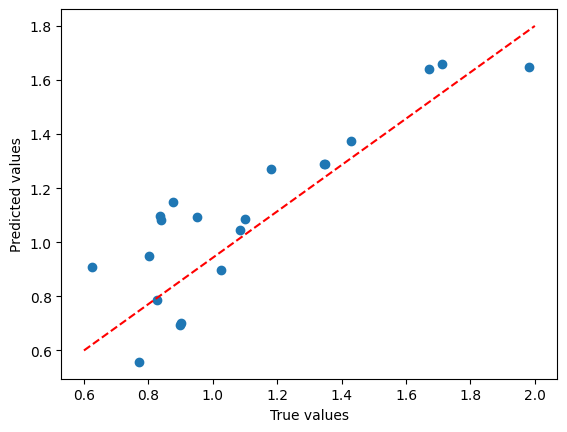
\includegraphics[width=1\linewidth]{images/serie_A_linear_reg.png}
    \caption{Plotted Predicted Goals per 90 against Actual Goals per 90}
    \label{fig:serie_A_linear_reg}
\end{figure}

\section*{Comparison Across Leagues}
We can extend our methodology beyond Serie A to the other four leagues, analyzing how homology impacts scoring with different playing styles and tactical approaches involved. 

For example, as detailed above, leagues like Serie A utilize compact team formations and counterattacking play, which produces passing networks with fewer and more isolated clusters. In contrast, leagues like La Liga that emphasize fluid, high-possession styles may exhibit passing networks with more interconnected nodes and higher loop counts, indicative of sustained ball circulation and intricate passing sequences. 

Variations in playing styles across leagues could influence the persistence statistics of passing networks in distinct ways, resulting in unique correlations between these statistics and scoring outcomes and making the number of goals scored easier to predict in certain leagues as compared to others. Potential limitations in our methodology that also could have accounted for variations or inconsistencies in the data are addressed in the next section.

The passing networks below represent Sampdoria in the 2015/2016 Serie A season and Barcelona in the 2015/2016 La Liga season, respectively.

\begin{figure}[H]
    \centering
    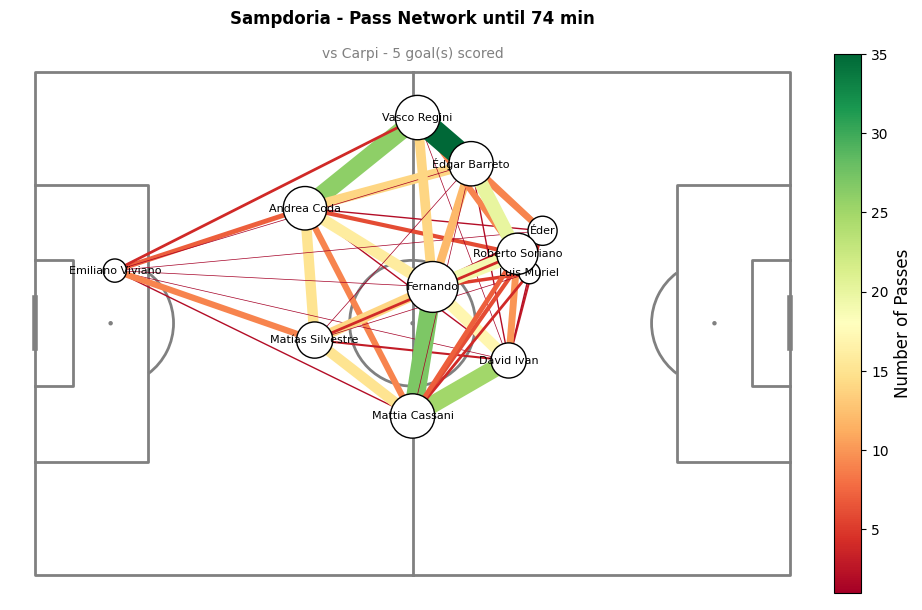
\includegraphics[width=1\linewidth]{images/SerieA.png}
    \caption{Passing Network of Sampdoria, against Carpi}
    \label{fig:SerieA_passing_network}
\end{figure}
\begin{figure}[H]
    \centering
    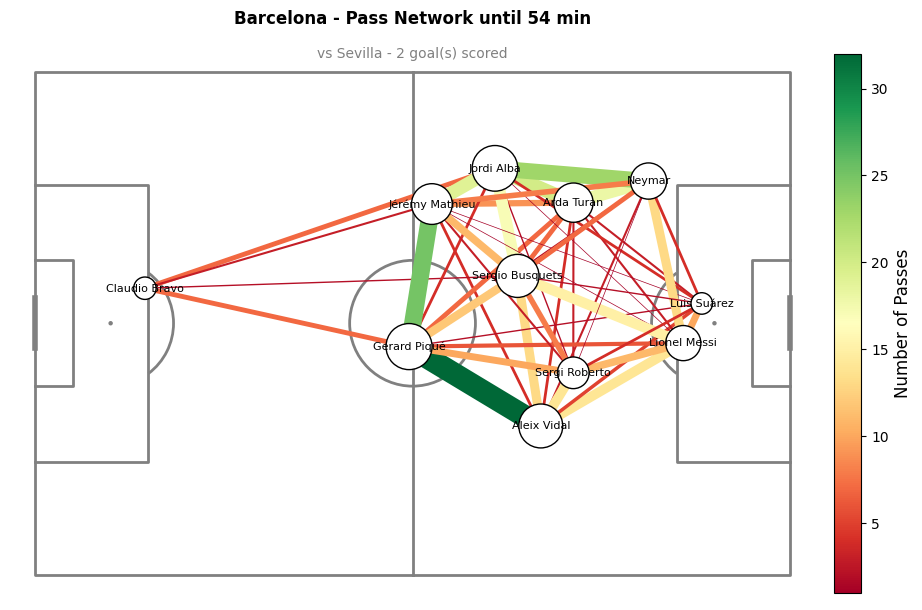
\includegraphics[width=1\linewidth]{images/LaLiga.png}
    \caption{Passing Network of Barcelona, against Sevilla}
    \label{fig:LaLiga_passing_network}
\end{figure}

Based on our methodology, we can obtain the correlation between each of the four persistence statistics and the target we are trying to predict (goals per 90), for each league. Additionally, we can calculate the $ R^2 $ of the linear regression that uses the four statistics to predict the target. The resulting table is below:

\begin{table}[H]
\centering
\renewcommand{\arraystretch}{1.3} % Adjust row height for readability

\scriptsize % Reduce font size for the table
\begin{tabular}{|p{1.2cm}|p{0.8cm}|p{0.8cm}|p{0.8cm}|p{0.8cm}|p{0.8cm}|}

\hline
\textbf{League} & \textbf{Avg Life $ H_0 $} & \textbf{Avg Life $ H_1 $} & \textbf{Std Life $ H_0 $} & \textbf{Std Life $ H_1 $} & \textbf{Reg R\textsuperscript{2}} \\ \hline
Bundesliga      & -0.334          & -0.283          & 0.412           & -0.053         & 0.437         \\ \hline
Premier League            & -0.337          & -0.123          & -0.155          & -0.229          & 0.184         \\ \hline
Serie A         & -0.483          & -0.472          & -0.226          & -0.210         & 0.642        \\ \hline
La Liga         & -0.303          & -0.422         & 0.511           & -0.289         & 0.606        \\ \hline
Ligue 1         & 0.143           & -0.520         & 0.327           & -0.338         & 0.346        \\ \hline
\end{tabular}
\caption{Correlation and Regression Analysis Across Leagues}
\label{tab:league_analysis}
\end{table}

\subsection*{Analysis}
The table demonstrates that, as expected, the predictability of goal-scoring outcomes varies significantly across leagues. 

In Serie A, the persistence statistics have the strongest relationship with the number of goals scored, with the linear regression model explaining $64.2\%$ of the variance. The average life length of $ H_0 $ has a correlation of $-0.483$ with goals, while the average life length of $ H_1 $ shows a correlation of $-0.472$, both indicating moderate negative relationships. These results suggest that passing networks characterized by less repetitive passing patterns and more cohesive connectivity are associated with improved scoring opportunities. This finding aligns with Serie A’s strategic style, which often emphasizes structured defensive setups and counterattacking play, relying on individual skill during offensive sequences to find the back of the net.

La Liga shows similar correlations for the average life lengths of $ H_0 $ and $ H_1 $ with goal-scoring outcomes. However, the correlation between the standard deviation of the life length of $ H_0 $ and goals was a lot higher than other leagues, reaching 0.511. This positive correlation suggests that greater variability in team connectivity create more goal-scoring opportunities. This finding highlights the Spanish league's fluid and adaptive style, where versatility and the ability to adjust passing dynamics across different matches play a critical role in creating scoring chances. Overall, the linear regression model performs well for La Liga, achieving an $ R^2 $ value of 0.606.

The Bundesliga shows weaker correlations between persistence statistics and goal outcomes compared to Serie A and La Liga. The standard deviation of the life lengths of $ H_0 $ is the only feature with a meaningful correlation with goals, reinforcing the idea that leagues with more dynamic and fast-paced gameplay require adaptability in passing structures to succeed.

In Ligue 1, the persistence statistics reveal some unique characteristics. The average life length of $ H_0 $ has a correlation of 0.143 with goals, making it the only league with a positive correlation for this feature. This suggests that less cohesive structures—indicative of fragmented networks—may be advantageous for goal scoring in France. Additionally, the average life length of $ H_1 $ has the most negative correlation among all leagues, highlighting the negative role of stable passing triangles in this league. These observations indicate the importance of individual skills in Ligue 1, where players like Ibrahimović, Cavani, and Di Maria often create and convert scoring opportunities themselves.

Finally, the Premier League presents the greatest challenge for predictability, with the linear regression model achieving an $ R^2 $ of only 0.184. This result suggests that the Premier League’s competitive and diverse tactical approaches lead to highly variable and adaptable passing structures, making it more difficult to link persistence statistics directly to goal-scoring outcomes.


\subsection*{Summary of Results}
Serie A showed the strongest correlation between persistence statistics and the number of goals scored, while the Premier League showed the least correlation. 

Due to differences in playing styles, tactical preferences, or other factors, a single pattern between the life lengths of $ H_0 $ and $ H_1 $ and the number of goals scored cannot be generalized across all leagues. However, the most useful statistic overall was the average life length of $ H_1 $, which seemed to remain the most consistent across all leagues.

\section*{Limitations}

Several limitations of our analysis that could have impacted our results must be acknowledged:

\begin{itemize}
    \item \textbf{Loss in Positional and Directional Information:} Using persistence means we sacrificed all spatial information. We did not account for the player's average position and the distance from other players, for example, which plays a role in the passing network and could have impacted the number of goals. Furthermore, we summed the passes between two players to have a less sparse dataset, losing information about the direction of passes.
    
    \item \textbf{Passing Networks Restricted to Early Match Minutes:} We constructed passing networks only up until the first substitution. This decision was made to avoid adding new nodes to the graph, which would complicate the structure. However, it excludes important later phases of the match, including tactical adjustments and substitutions, potentially omitting significant changes in team dynamics.
    
    \item \textbf{Standardized Goals Estimate:} To standardize goals scored, we projected the scoring rate up to the first substitution across a full 90 minutes. While this approach ensures comparability, it assumes a constant scoring rate, which may not reflect a team's true performance over the course of a match.
    
    \item \textbf{Exclusion of Red Cards:} We did not account for red cards in our analysis. An early red card would remove a player from the field, effectively excluding them from the passing network. This could drastically alter the team’s structure and performance but was not captured in our methodology.
    
    \item \textbf{Skewed Dataset:} Since many matches in the dataset recorded $0$ goals scored, the data is skewed towards $0$. This imbalance may bias the regression models and limit their ability to generalize, particularly in predicting matches with higher goal totals.
    
    \item \textbf{Limited Data Scope:} We included only leagues and seasons for which we had complete data for the entire season. While this ensured consistency, it restricted our analysis to a limited dataset. Access to more leagues and seasons could provide a broader perspective and more robust results. Also, inferring and drawing conclusions about a league from just a single season is not the most reliable, as it fails to account for variability across seasons, changes in team compositions, tactical evolutions, and other dynamic factors that influence league-wide trends. 
    
    \item \textbf{Passing is Not All of Soccer:} Finally, our analysis focused exclusively on passing networks. While passing is a critical aspect of soccer, many other factors such as set pieces, individual skill, defensive tactics, team morale, and physicality contribute to scoring and overall performance. Thus, not all aspects of the game can be fully explained by passing metrics alone.
\end{itemize}

These limitations highlight the challenges of analyzing complex team sports like soccer and suggest several avenues for future research, including the incorporation of additional data, accounting for red cards, and integrating other aspects of the game beyond passing.

\section*{Conclusion}

In this study, we applied TDA to soccer passing networks to investigate the relationship between network topology and goal-scoring outcomes. By extracting data from Europe’s top five leagues during the 2015/2016 season, we utilized persistence statistics based on the life lengths of $ H_0 $ and $ H_1 $ to quantify team connectivity and passing loops. We plotted the correlation between the average and standard deviation of these life lengths against the number of goals scored, drawing conclusions about how network cohesiveness, consistency, and variability affect scoring in different leagues with different styles of play. We further used a regression model to analyze how much the scoring outcome depends on these persistence statistics. 

Our findings revealed league-specific correlations between homological features and scoring, with Serie A showing the strongest predictive relationship. On the other hand, the Premier League presented more variability and is very hard to predict, potentially due to the diversity in tactics. Interestingly, the average life length of $ H_1 $ contributed most consistently to the relationship between homology and the number of goals scored across all leagues.

Despite limitations like the loss of positional information and the focus on early match phases, the research highlighted the potential of TDA for understanding team dynamics and performance in sports. Future work can expand the data scope, incorporate additional game factors, and refine methodologies to build on these findings.
\newpage
\printbibliography

\begin{quote}
\end{quote}

\end{document}

